\documentclass[runningheads,a4paper]{llncs}

\usepackage{graphicx}
\usepackage{subfigure}
\usepackage[utf8]{inputenc}
\pagenumbering{roman}
\usepackage{textcomp}
\usepackage{pifont}
\usepackage{color}
\usepackage{blindtext}
\usepackage{enumitem}


\begin{document}
\mainmatter  % start of an individual contribution

%Titel
\title{HCI Meilenstein 1}

\titlerunning{HCI Meilenstein 1}

\author{
  Dursun, Camkerten
  \texttt{a0027244@@unet.univie.ac.at}
  \and
  Pektas, Tarik
  \texttt{a1325165@@unet.univie.ac.at}
  \and
  Bozkurt Yigit Berkay
  \texttt{a1029659@@unet.univie.ac.at}
  \and
  Ayyildiz Mert Ahmet
  \texttt{a1125172@@unet.univie.ac.at}
}

\institute{Universität Wien  / HCI \\
\ SS16 / Gruppe 3}


\maketitle

\section{Wahl des Themas}
\textbf {Projekt 14: Meine Finanzen}\\

Wir sind der gleichen Auffassungen, wie in der Projektbeschreibung des Projektes 14 beschrieben, dass neuen Technologien im Finanzsektor sehr stark im Trend sind. Deshalb haben wir uns für dieses Projekt entschieden. Wir denken dass dieses Projekt, uns eine erfahrungsreiche Einsicht in die Branche sowie eine solide Grundlage für spätere Entwicklungen geben wird. \\\\Das Hauptziel der Applikation wird  es sein, die Finanzen des Nutzers zu verwalten sowie mit entsprechenden Berichten die Übersicht visuell darzustellen. Wichtig hierbei ist es, das die Möglichkeit besteht einzelne Ausgaben zu etikettieren um bei der Visuellen Darstellung, eine auf dem ersten Blick verständliche Finanzsituation, per Auflistung der Ein und Ausgaben zu wiedergeben. 


\section{Diskussion von relevanter Literatur}

\subsection{Design and Implementation Money Management Web Based Application for Personal and Family Proposed for CV. X  [1]}
Mittelklasse Verbraucher haben nicht genug Zeit, um ihre persönlichen Finanzen zu verwalten. Einige von ihnen sind nicht fähig, um ihr Einkommen und das Ergebnis zu verwalten. Obwohl sie erkennen, dass sie professionelle Beratung benötigen, wollen sie nicht die persönliche Finanzberatung bezahlen, weil ihre Kosten relativ teuer. Sie fordern einfach und schnell Geld- Management- Dienstleistungen. Die Mittelklassen sind derzeit sehr abhängig von ihren Smartphones. Diese sind nicht nur für die Kommunikation, sondern sie können auch ihren Lebensstil verbessern. Grundsätzlich Menschen brauchen, Instant und einfach Lösungen um ihre finanziellen Probleme zu lösen.\\ Eine andere Behauptung in der Artikel steht ist, dass die Mittelklasse  wenig Zeit hat, um ihre Finanzen zu sorgen. An Wochentagen Menschen haben nur 3 Stunden pro Tag für persönliche Aktivitäten. Es ist auch über Vorbereitung des Projekts und seine Analysen viel erwähnt. Durch die Artikel hat unsere Team die genauere Anforderungen von Konsumenten besser versteht. Es beinhaltet auch vielfältige Informationen über den Entwicklung-Prozess der Applikation.     


\subsection{How to Choose and Use Financial Software [2]}
Die Text beinhaltet Informationen über Software-Wahl und wichtige Ratschläge für Benutzer. Es informiert auch über Steuer-Vorbereitungsprogramme und Web-basierte Geld-ManagementWebseiten. 
 Unser Team hat die Wichtigkeit der Sicherheit und Geheimhaltung besser verstanden. Die Benutzer suchen immer Preisnachlass und weitere Aktionen, deswegen werden wir Gutscheincodes oder Rabatte anbieten, damit wir meist verwendete Applikation werden kann.   

\subsection{Personal Finance Software Reviews [3]}
Obwohl alle persönliche Finanz-Software eine Zeitaufwand braucht und manche benötigen manuelle Daten-Import, die besten Programme sparen Zeit für die Benutzer durch die Synchronisation mit Ihrem Finanzinstitutionen und unterstützt in Echtzeit Zugriff auf Ihre Daten. Die besten Programme synchronisieren auch mit mobilen Apps um Ihr Finanzielle Situation zu überwachen. 
Fast alle Applikationen umfasst Budgetierung und Reporting-Tools. Eine mögliche Vorteil, die Benutzer Maximum an Flexibilität bei der Verfolgung und Ausgabe Kategorisierung. \\Die Applikation soll auch ermöglichen, die Kontodaten manuell in gängigen Formaten importieren, wie Excel oder CSV, in dem Fall, dass Sie nicht online sind, auf Ihre Konten über die Software zu verbinden. Die 
Benutzer wollen auch sicherstellen, dass die Software-Sicherheitsfunktionen wie Verschlüsselung und Kennwortschutz enthalten.\\ Die Rezension hat unsere Aspekte erweitert z.B. Was sollten Benutzer erwarten von Personal Finanz Software. Team kann jetzt die Anforderungen der Benutzer besser erkennen.  

\subsection{The Best Personal Finance Software [4]}
Eine gültige Besorgnis über eine persönliche Finanz-App ist die Sicherheit. Ehrlich gesagt, die meisten der Namen Marke Anwendungen empfehlt sind, wahrscheinlich so sicher wie eine Kreditkarte in Ihrer Brieftasche. Normalerweise verwenden persönliche Finanz-Websites und Programme 128-BitBankebene oder 256-Bit-Militär-Level-Verschlüsselung und von TRUSTe, VeriSign und McAfee verifiziert werden. \\ Wir haben empfohlene Applikationen getestet und jetzt wir haben jetzt mehr Ideen über Bedienoberflächen und Nutzbarkeit. Ein andere wichtige Thema ist, dass die unsere Finanz Applikation soll von Security Firmen verifiziert sein.
\clearpage

\section{Analyse \& Diskussion von Konkurrenzprodukten}
\subsection{App Meine Finanzen[5]}

\begin{itemize}
\item \textbf {Funktionalität}: \\\\
Die für iPhone und iPad konzipierte Applikation bietet auch Apple-Watch App. Einnahmen und Ausgaben von mehreren Konten können mit Hilfe der App festgehalten werden. Neben zeitgleiche Transaktionen können auch Buchungen einmalig oder wiederkehrend geplant erstellt werden. Durch Kategorien können alle Transaktionen gruppiert werden.  Mit einem 4-stelligen Code oder mit einem TouchID (falls unterstützt) können die Daten gegen Fremdzugriff geschützt werden. \\

Im Gratisversion können 20 Buchungen pro Monat festgehalten werden.  Daten können im Gratisversion importiert werden, Statistiken, Datenexport und automatische Backups können jedoch nur bei Erwerb der Vollversion durchgeführt werden.\\


\item \textbf {Usability}: \\

\textcolor{green}{\ding{51}}	Die Applikation ist leicht zu bedienen. \\
\textcolor{green}{\ding{51}}	bietet eine Anleitungsvideo und Hilfe-Dokumentation auf der Homepage\\
\textcolor{green}{\ding{51}}	Support-Email für eventuelle Fragen vorhanden.\\
\textcolor{red}{\ding{55}}	keine individuellen Kontenansicht

\end{itemize}


\begin{figure}
\centering
\subfigure[MeineFinanzen App]{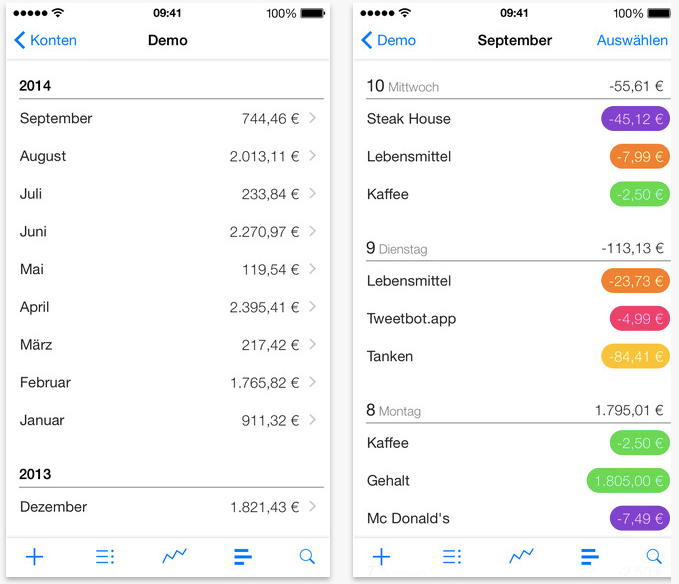
\includegraphics[height=7cm,width=8cm]{meineFinanzen}}
\end{figure}
\clearpage



\subsection{App Moneyboard Pro [6]}
\begin{itemize} 
\item \textbf{Funktionalität}: Moneyboard gibt es für iPhone, iPad und iPod touch. Mit der Finanzapplikation können Einnahmen und Ausgaben verwaltet werden. Transaktionen können nach Woche, Monat oder Jahr gefiltert werden.  Für jede Buchung kann auch ein Belegfoto hinterlegt werden. \\

Im Rahmen eines Gratisversions  kann nur ein Konto mit unbegrenzten Transaktionen festgehalten werden.  Neue Kategorien und Datenexport ist nur im Vollversion möglich.\\\\

\item \textbf{Usability}:\\

\textcolor{green}{\ding{51}}	Konten können mit Profilfoto und Farben individualisiert werden\\
\textcolor{green}{\ding{51}}	Kategorien können mit Symbolbild (icon) veranschaulicht werden\\
\textcolor{green}{\ding{51}}	dynamische Grafiken verstärken die Visualität.\\
\textcolor{red}{\ding{55}}	Sprache: Übersetzung in deutsche Sprache teilweise falsch oder nicht vollständig.\\
\textcolor{red}{\ding{55}}	"Ausgabe" wird auch als Auslage sowie expenses verwendet. \\
\textcolor{red}{\ding{55}}	Schreibfehler (Edigieren statt Redigieren (Korrektur))\\
\end{itemize}


\begin{figure}
\centering
\subfigure[Moneyboard Pro App]{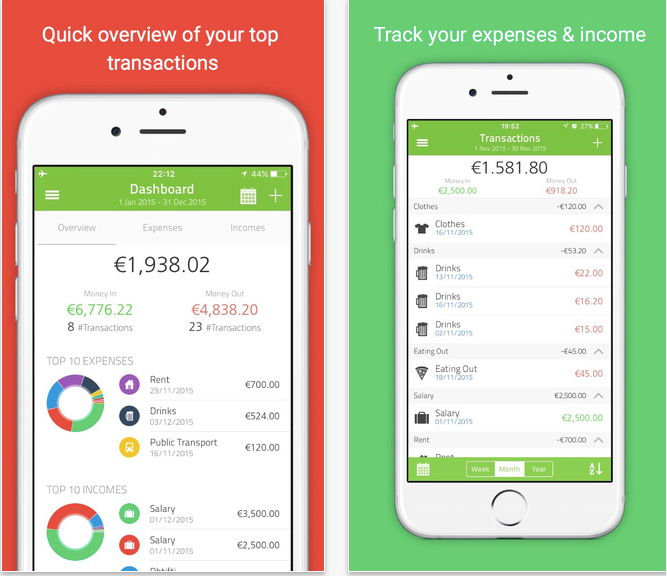
\includegraphics[height=7cm,width=8cm]{moneyboard}}
\end{figure}

\clearpage

\subsection{Haushaltsbuch Pro [7]}
\begin{itemize} 

\item\textbf{Funktionalität}\\
Mit der App gibt es die Möglichkeit ein Haushalt zu erstellen und es mit anderen Nutzern zu teilen, um die Einnahmen und Ausgaben für einen Haushalt gemeinsam zu verwalten. Durch Familien-Synchronisation haben alle Mitglieder des Haushalts Zugriff auf die selben Transaktionen. \\
Im Gratisversion können nur 5 Transaktionen pro Tag erstellt werden. Die App gibt es für iPhone, iPad und iPod touch und bietet auch Apple-Watch App.\\

\item\textbf{Usability}\\

\textcolor{green}{\ding{51}}	Feedback nach Erstellung einer Transaktion\\
\textcolor{green}{\ding{51}}	dynamische Grafiken\\
\textcolor{red}{\ding{55}}	Keine Hilfe-Dokumentation\\

\end{itemize}

\begin{figure}
\centering
\subfigure[HaushaltsPro App]{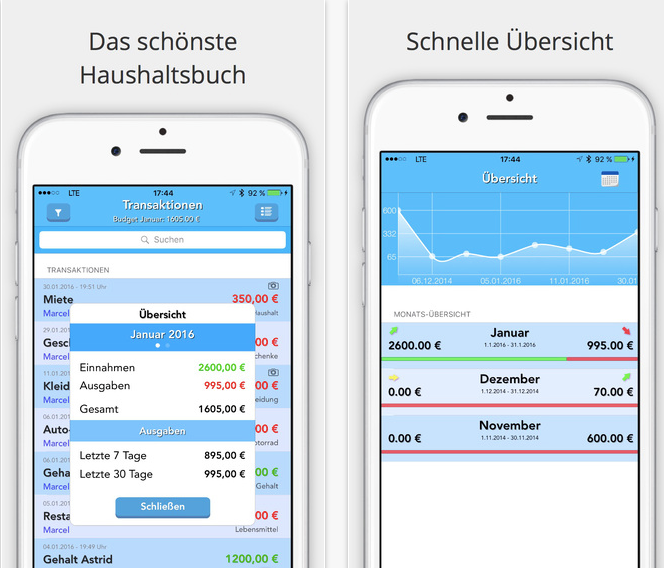
\includegraphics[height=7cm,width=8cm]{haushaltsbuchPro}}
\end{figure}
\clearpage


\subsection{Übersicht der analysierten Applikationen}

\begin{figure}
\centering
\subfigure[Vergleich]{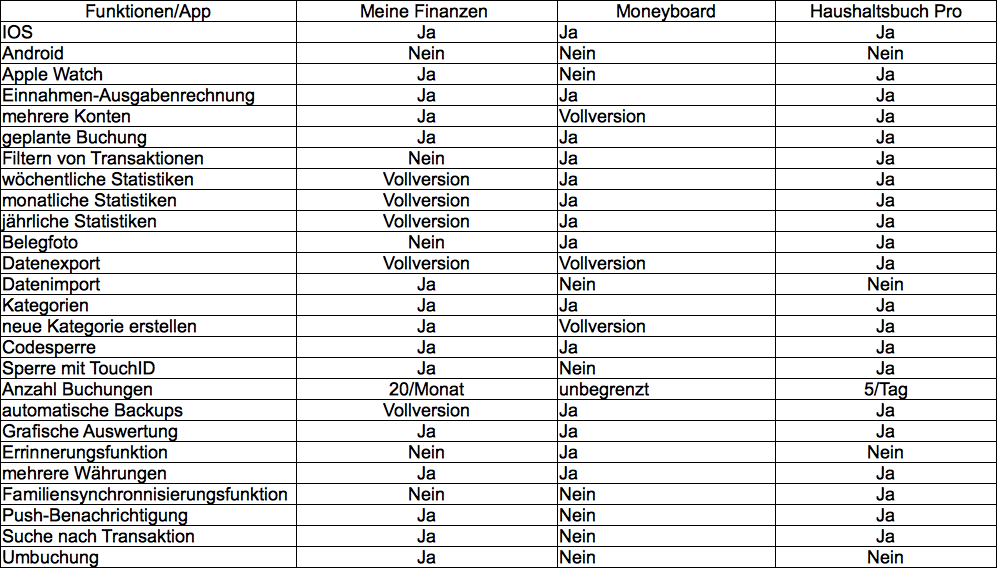
\includegraphics[height=12cm,width=13cm]{ubersicht}}
\end{figure}
\clearpage

\section{Nutzeranalyse (User Analysis)}
\subsection{Übersicht Benutzergruppen}


\textbf{Primär} Erwachsene Personen mit einem durchschnittlichem Einkommen, \\ Familienoberhaupt\\
\textbf{Sekundär} Sachwalter, Buchhalter\\
\textbf{Grenzfälle} Jugendliche unter 16, Ältere Personen über 60\\

\subsection{Beschreibung der Benutzergruppen}

\textbullet \textbf{ Primäre Benutzergruppen}\\
Unsere App wird mit hoher Wahrscheinlichkeit von Erwachsenen Personen, mit einem durchschnittlichen Einkommen, öfters in Anspruch genommen da nun mal für diese Gruppe eine genaue Auflistung, insbesondere der Ausgaben,  sicherlich interessanter ist. Eine kontinuierliche Überwachung der Ein- und Ausgaben kann unter Umständen auf längere Zeit viele unnötige Kosten aufdecken und somit die Lebensqualität, dank einer konkreteren Aufteilung der Finanzen, erheblich steigern.\\
Eine weitere Primäre Nutzergruppe, ungeachtet der Einkommenshöhe, wären Familien-Väter/ Mütter, die die Verantwortung einer gerechten Aufteilung des Einkommens innerhalb des Familienkreises gewährleisten. Auch diese Gruppe würde sicherlich dank der Übersicht welcher unsere App gewährleisten wird sehr profitieren.\\

\textbullet\textbf{ Sekundäre Benutzergruppen}\\
Da wir in unserer App, spätestens in den erweiterten Versionen, eine Multiuser Umgebung implementieren werden, so das ein Nutzer auch mehrere Konten verwalten kann, könnte dies die  Interesse bestimmter Berufe wecken, zumal eines Sachwalters. Ein Sachwalter, unter dessen Aufgaben zumeist auch die Verwaltung eines Vermögens fällt, könnte dank unserer App diesen mit Leichtigkeit betreuen und hätte ein Abbild der Ist-Situation immer griffbereit. \\\\
Eine andere Benutzergruppe könnten Buchhalter sein. Natürlich kann unserer App nicht all die umfangreichen Funktionen einer Buchhaltungssoftware abdecken, dennoch wird Sie in der Lage sein die alltäglichen Finanzbewegungen einer Privatperson zur decken.  Dies könnte bei kleinen Einzelunternehmen in der Startphase sicherlich interessant sein. \\


\textbullet \textbf{ Grenzfälle}\\
Da eine "Finanzensteuerung" zumindest einen gewissen Grad an Verantwortungsbewusstsein voraussetzt, ist es weniger zu erwarten, dass Personen unter 16 Jahren, sich für unsere App interessieren. Selbst bei sehr vielen verantwortungsbewussten Jugendlichen, gäbe es wohl aufgrund der eingeschränkten Finanzen trotzdem es keinen Bedarf an unserer App. \\
Bei älteren Personen, insbesondere über 60, denken wir dass der Umstieg von Blatt Papier und Stift selbst bei noch so großartiger "Usability" sehr schwer sein wird. Natürlich wird es auch hier Ausnahmen geben.  



\section{Personas}
\subsection{Primär Persona: Thomas STEIGER - \\Person mit einem durchschnittlichen Einkommen}

\begin{figure}
\centering

\includegraphics[height=3cm,width=3cm]{thomasSteiger}
\caption{Thomas Steiger[8]}

\end{figure}
                                          
\textbf{Info und Freizeit}: \\
Thomas (23) studiert an der Uni Wien und neben dem Studium arbeitet als Kellner. Er wohnt mit seiner beste Freund in einer Wohnung. Sein bestes Hobby ist um Natur zu fotografieren. Als Freizeit Aktivitäten macht er gerne trainieren, lesen und Schah spielen. Er geht mit seinem Freund Minimum einmal zu einem Event (Kino, Ausstellung, Disco, Theater usw.) \\\\
\textbf{ Ziele, Wünsche, Erwartungen}\\ • Dieser Student sollte seine Einkommen und Ausgeben wissen und seine Erfolgsrechnung mit dem einfachsten Weg sehr gut anrechnen.\\\\
• Er hat ein Ziel, die ein neuen Fotoapparat zu haben. Mit diesem Finanz App kann er rechnen, wie viel und wie lange für dieses Ziel sparen muss.\\\\
• Daneben ist es simple alle Ein und Ausgaben zum Kontrollieren. Er braucht kein Papier nur mit eigenes Smartphone und es dauert jeden Tag Maximum 1-2 Minuten.  In diesem Technologie Zeit passt diesem Finanz App für diese Junge Student sehr antreffend.\\
 Ich habe als Vorbild Thomas ausgewählt, da die jugendliche Leute Smartphone bevorzugen, statt die Schreibwaren zu benutzen. 


\clearpage

\subsection{Primär Persona: Julian Kuhlbert - \\Familienvater}

\begin{figure}
\centering

\includegraphics[height=4cm,width=6cm]{juliankuhlberg}
\caption{Julian Kuhlbert [9]}

\end{figure}
                                          
\textbf{Info und Freizeit}: \\
Julian (48) ist ein Rechtsanwalt. Seit 7 Jahren ist er verheiratet und hat 2 Kinder. Kuhlbert Familie lebt in einer Größeren Wohnung in Wien. Vater Julian probiert in der Technologiezeit dar einzufügen. Er hatte kein Interesse an der Technologie.
In seiner Freizeit würde er gerne Tennis spielen, lesen, pirschen.\\


\textbf{ Ziele, Wünsche, Erwartungen}\\

• Um Jedes Jahr irgendwo Urlaub zu machen, braucht Herr Julian eine Spar box Applikation in seinem Handy zu benutzen.\\\\
• Ein- und Ausgabe wurden von dieser Finanz Applikation errechnet. \\\\
• Er hat Bedürfnisse im Augenblick Ein und Ausgaben in dieser Finanz App zu speichern.\\\\
  Ich habe als Vorbild Julian ausgewählt. Obwohl er kein Interesse an der Technologie, kann er einfach diese Finanz App auf seinem Handy nutzen. Da dieser App sich an alle wendet.\\


\clearpage


\subsection{Sekundär Persona: Lena Bauer - \\Buchhalterin}

\begin{figure}
\centering

\includegraphics[height=4cm,width=5cm]{lenabauer}
\caption{Lena Bauer[10]}

\end{figure}
                                          
\textbf{Info und Freizeit}: \\
Lena (30) ist eine Buchhalterin.Sie ist verheiratet seit 7 Jahren und hat 1 Kind. Lena lebt mit ihrer Familie in einem Größeren Villa in Wien. Sie verdient sehr gut und kontrolliert ihre Ein und Ausgaben nicht häufig. \\\\
In seiner Freizeit würde sie gerne mit seiner Familie verbringen, außerdem macht sie gerne puzzle. Sie hat Große Puzzle Collection. \\\\



\textbf{ Ziele, Wünsche, Erwartungen}\\

• Um Jede Woche Special Puzzle zu kaufen, braucht Frau Lena eine Spar box Applikation in seinem Handy zu benutzen. \\\\
• Ein- und Ausgabe ist nicht wichtig für sie von dieser Finanz Applikation zu errechnen. \\
Ich habe als Vorbild Lena ausgewählt. Obwohl sie noch schwerere Finanz Programme Kenntnisse hat, ist diesem Finanz App für sie sehr leicht geworden. \\
Sie ist ganz genau unsere Sekundäre Persona.
\clearpage

\subsection{Negativ Persona: Wilhelm Kastner - \\Ältere Person}

\begin{figure}
\centering

\includegraphics[height=4cm,width=5cm]{wilhemkastner}
\caption{Wilhelm Kastner[11]}

\end{figure}
                                          
\textbf{Info und Freizeit}: \\\\
-Wilhelm (77) war Mathe Professor an der Universität Berlin. Er ist jetzt Pensionist.\\
-Er wohnt alleine einer Wohnung in Berlin. Sein bestes Hobby ist jeden Tag um Rätsel zu lösen. Als Freizeit Aktivitäten macht er gerne lesen und Schah spielen. Er geht mit seinem beste Freund Minimum einmal indem Tag zu spazieren.  \\\\



\textbf{ Ziele, Wünsche, Erwartungen}\\

• Er muss nicht seine Einkommen und Ausgeben wissen und seine Erfolgsrechnung anrechnen. Daneben hat er kein Smartphone oder Tablet.\\
• Er hat kein Ziel und kein Interesse an der Technologie.\\

In diesem Technologie Zeit passt diesem Finanz App für Herr Wilhelm nicht. Ich habe als Vorbild Wilhelm ausgewählt, da die älteren Leute die Schreibwaren bevorzugen, statt die Smartphone oder Tablet zu benutzen. 

\clearpage

\section{Aufgabenanalyse}
\subsection{Was tut unsere App ?}
\begin{itemize}
\item Mit der Finanz App können Sie Ein- und Ausgaben verwalten.
\item Es ist Möglich ein Haushalt erstellen und es zu teilen
\item Wenn Sie eine Gruppe gründen, dann können Sie mit dem ganze Familie in diesem gruppe zusammen diskutieren oder melden
\item Mit dieser Finanz App können Sie rechnen, wie viel und wie lange für Ihr Ziel sparen
\item Es ist Simple alle Ein- und Ausgaben zum Kontrollieren.
\item Man hat Bedürfnisse im Augenblick Ein- und Ausgaben in dieser Finanz App zu speichern
\end {itemize}

\subsection{Wieso unsere App ?}
\begin{itemize}
\item Diese Finanz App ist sehr simple zu benutzen
\item Nur mit einem Anruf oder per E-Mail haben Sie technischen Unterstützung.
\item Sie können ein Profilfoto erstellen und für alle Aus- und Eingaben Farbe initialisieren
\item Gute Qualität
\item Dynamische Grafiken
\item Für jede Ein- und Ausgaben können Sie neben dem Betrag etwas notieren
\end {itemize}


\begin{figure}
\centering
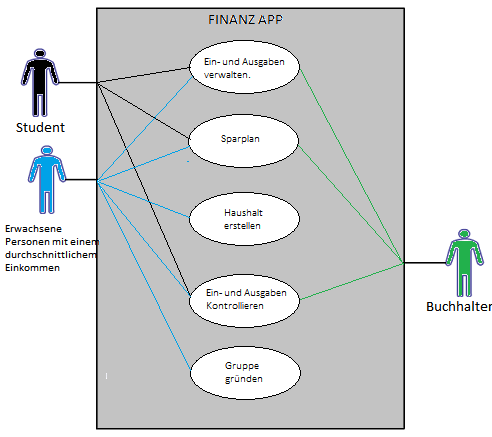
\includegraphics[height=7cm,width=15cm]{usecase}
\caption{Usecase Diagram]}
\end{figure}
\clearpage
                     

\subsection{Taskanalyse}

\begin{figure}
\centering
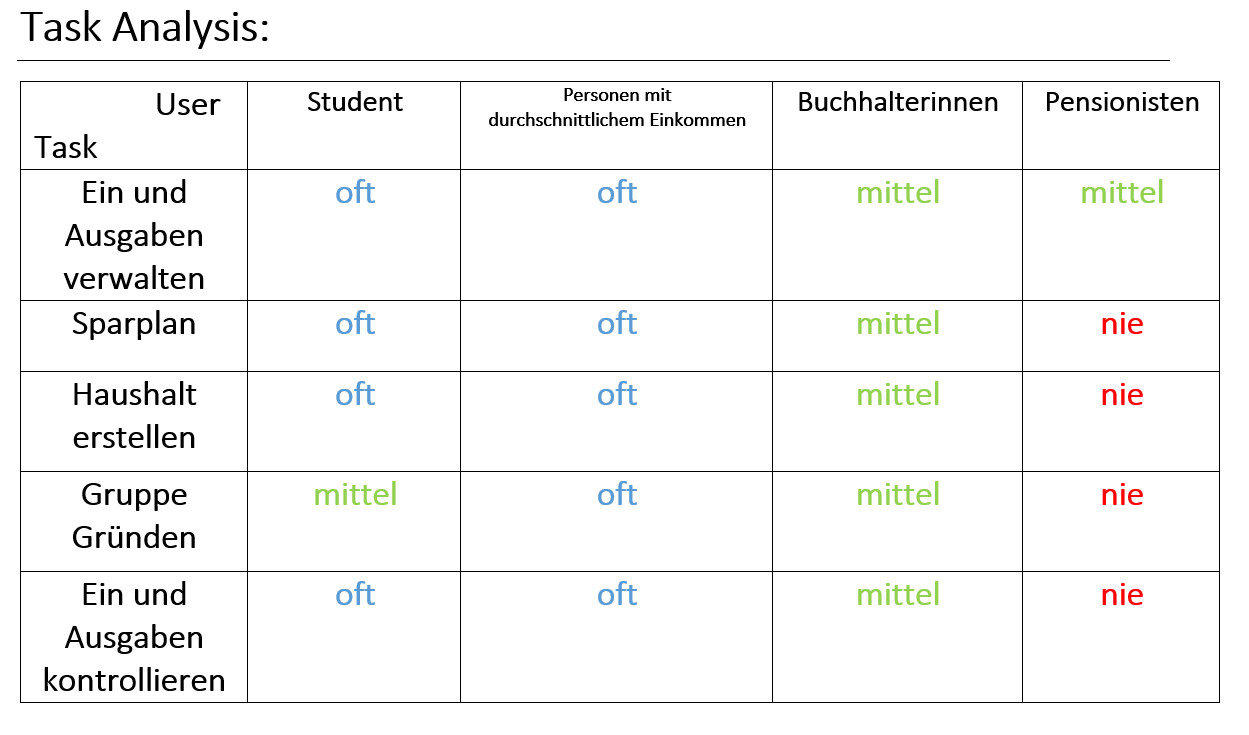
\includegraphics[height=10cm,width=13cm]{aufgabenanalyse}
\caption{Task Analyse}
\end{figure}
\clearpage

\section{Kontextanalyse}

Wir denken dass unsere App in einer ruhigen Verfassung benutzt wird. Es ist wohl unüblich Finanzen in Hektik zu verwalten. Die Umgebung wird sich allerdings sehr oft ändern. Wir gehen davon aus das die Einnahmen öfters zuhause beziehungsweise auch im Büro eingetragen werden. Die Ausgaben allerdings könnten sehr wohl gleich nach einem Einkauf eingegeben werden. Da dies wahrscheinlich im Stehen oder unterwegs sein wird muss diese Eingabe besonders leicht zu tätigen sein. \\\\Vielleicht wäre angesichts dessen ein Feature, wie zum Beispiel ein "Einkauf getätigt" Button angebracht, welcher zur einen späteren Zeitpunkt die App veranlasst den Nutzer an die unvollständige Aktion zu erinnern. Generell sollte die App eher täglich verwendet werden als ein wöchentlich oder gar monatlich. Ziel sollte es sein jede Bewegung sofort abzubilden. 


\section{Projektmanagement}
\subsection{Kontext}
Entwicklung einer App namens "Meine Finanzen" das die Ein und Ausgaben eines Nutzers abspeichert, kategorisiert und visuell wiedergibt. Entsprechende Berichtsfunktionen, basierend auf Zeitraum und Kategorien, ausgeben und in Bezug auf das Verhalten dynamische Tipps generieren kann.

\subsection{Motivation}
Der Finanzdienstleistungsbereich ist offensichtlich im stark steigenden Trend. Dies liegt insbesondere daran das viele Menschen heutzutage ihr Hauptaugenmerk auf ihre Finanzen richten. Ungeachtet dessen, ob nun richtig oder falsch, ermöglicht dies, im Zusammenhang mit Smartphones welche schon seit längerem ein unverzichtbarer Teil unseres Lebens sind, neue Möglichkeiten. Möglichkeiten diesen Bedarf an Übersicht, sowie an einem dynamischen Ratgeber und eine kontinuierliche Kontrolle der Finanzen durch eine App zu gewährleisten.\\ Unsere Motivation ist es diesen Bedarf abzudecken. Ein Geschäftsmodell können wir uns durch die "Subscriptions"  oder aber auch Free2use im Gegenzug von Austausch von Daten vorstellen. Diese wären dann wiederum, natürlich anonymisiert, für viele Institute interessant. 

\subsection{Ziele}
•	Ein und Ausgaben abbilden\\
•	Budgetierung ermöglichen\\
•	Etikettierung \\
•	Finance Advisor (Tipps entsprechend Ausgabeverhalten)\\
•	Fertigstellung der App bis 08.06.2016\\


\subsection{Nicht-Ziele}
•	Bankapplikationen zu ersetzen\\
•	Transaktionen durchzuführen (Gelüberweisungen etc.)\\
•	Ausschließlich als ein Ein-Ausgaben Rechner dienen\\



\subsection{Das Projektteam stellt sich vor}
\subsubsection{Ayyildiz Mert Ahmet}
studiert besucht nebem seinem Informatik Studium an der Hauptuniversität auch zugleich Software Informatik an der Technischen Universität.
Er lebt in der kleinen Gemeinde Bruck an der leitha.

\subsubsection{Bozkurt Yigit Berkay}
ist 22 Jahre alt und ist schon seit langem an der Informatik interessiert. Er lebt in Wien und besucht aktuell sein 3. Semester an der Universität.

\subsubsection{Camkerten Dursun,}
ist aktuell in einem Software Unternehmen im Bereich der Testautomation, als Entwickler beschäftigt. Zudem befindet er sich, in seinem berufsbegleitenden Studium der Medien Informatik an der Universität Wien, im 5. Semester. 


\subsubsection{Pektas Tarik,}
Vater einer sehr lieben Tochter, studiert an der Universität Wien berufsbegleitend Wirtschaftsinformatik, im 3. Semester. Um sein Studium abzuschließen, pendelt er unermüdlich zwischen Wien und seinem Zuhause, welches in St. Pölten liegt, täglich hin und her.


\begin{thebibliography}{1}
\bibitem{proceeding1} Design and Implementation Money Management Web Based Application for Personal and Family Proposed for CV. X Mumpuni, Melvin ; Sukarno, Subiakto Procedia - Social and Behavioral Sciences, 2014, Vol.115, pp.444-459 [Peer Reviewed Journal] 
\bibitem{proceeding2} http://guides.wsj.com/personal-finance/managing-your-money/how-to-choose-and-use-financial-software
\bibitem{proceeding3} http://personal-finance-software-review.toptenreviews.com/
\bibitem{proceeding4} http://www.pcmag.com/article2/0,2817,2407617,00.asp
\bibitem{proceeding5} https://itunes.apple.com/at/app/meine-finanzen-personliche/id797005152?mt=8
\bibitem{proceeding6}https://itunes.apple.com/us/app/moneyboard-personal-finance/id625887028?mt=8
\bibitem{proceeding7} https://itunes.apple.com/at/app/haushaltsbuch-pro/id879507285?mt=8
\bibitem{proceeding8} http://www.dpsg-oesede.de/img/moritz.jpg
\bibitem{proceeding9} http://www.haaretz.com/polopolyfs/1.664893.1436288976!/image/3768882842.jpg
\bibitem{proceeding10} http://www.tcm-gyni.ch/wp-content/uploads/2013/04/schwangerchaftsbeschwerden-linderun.jpg
\bibitem{proceeding11} http://www.nkfu.com/wp-content/uploads/2011/07/yasli-adam.jpg

\end{thebibliography}


\end{document}